\documentclass{beamer} % {article} %
\usepackage{etoolbox}
\mode<presentation>
%\usepackage{beamerarticle}
%\usepackage{graphicx}



\usepackage{tikz}


\usetheme{Frankfurt}%
\usecolortheme{seagull}
\logo{
\includegraphics[height=.25in]{img/clarksonGreen}}

\definecolor{garnet}{RGB}{136,0,0}
%\definecolor{clarksonGreen}{RGB}{0,71,28}
\definecolor{clarksonGreen}{RGB}{0,52,21}
\setbeamercolor{palette primary}{fg=clarksonGreen,bg=white}
\setbeamercolor{palette secondary}{fg=clarksonGreen,bg=white}
\setbeamercolor{palette tertiary}{fg=clarksonGreen,bg=white}
\setbeamercolor{palette quaternary}{bg=clarksonGreen,fg=white}
\setbeamercolor{block title}{fg=black,bg=black!15}
\setbeamercolor{block body}{fg=black,bg=black!10}
\setbeamercolor{titlelike}{bg=clarksonGreen,fg=white} % parent=palette quaternary}

%\includeonly{introduction2ODEs}
%\includeonly{solutionsToDEs}


\begin{document}

\author{Amanda Groccia, Tatyania Moorehead, Carrie Rider}
\institute{University of Connecticut, Norfolk State University, Clarkson University}


% %%%%%%%%%%%%%%%%%%%%%%%%%%%%%%%%%%%%%%%%%%%%%%%%%%%%%%%%%%%%
% %%%%% The title page

\title{Stochastic Differential Equations}
\subtitle{Introduction}
\date{\today}

\begin{frame}
  \titlepage
\end{frame}


\begin{frame}
  \frametitle{Outline}
  \tableofcontents[hideallsubsections]
\end{frame}


% %%%%%%%%%%%%%%%%%%%%%%%%%%%%%%%%%%%%%%%%%%%%%%%%%%%%%%%%%%%%
% %%%%% The overview and introduction

\section{Background on Shrimpy}


\begin{frame}
  \frametitle{Outline}
  \tableofcontents[ currentsection ]
\end{frame}

\subsection{The Problem}

\begin{frame}
  \frametitle{The Problem}

  Southern German water routes have had several drastic population changes concerning gammarids. \\
\vspace{1em}
Much of this is due to canal construction. 

  \begin{columns}[t]
    \column{.45\textwidth} 
	\begin{block}{Native Species:}
    %\centerline{\includegraphics[height=5.0cm]{gainComp-001}} 
	\textit{Gammarus pulex (Gp)}
	\end{block}

    \column{.55\textwidth}
	\begin{block}{Invasive Species:}
    %\centerline{\includegraphics[height=5.0cm]{energyComp-001}}
    	\textit{Dikerogammarus villosus (Dv)}\\	
	\textit{Dikerogammarus haemobaphes (Dh)}\\
	\textit{Dikerogammarus bispinosus (Db)}\\
	\textit{Echinogammarus berilloni (Eb)}
	\end{block}
  \end{columns}
\end{frame}

\begin{frame}{Killer Shrimp}
\centerline{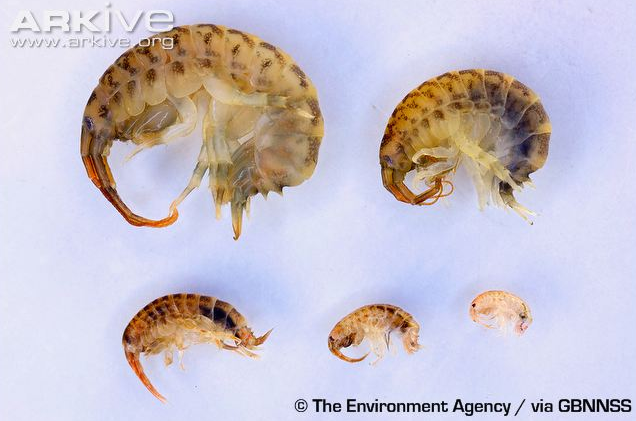
\includegraphics[width=8cm]{shrimpy1}}
\end{frame}

\begin{frame}{Killer Shrimp}
\centerline{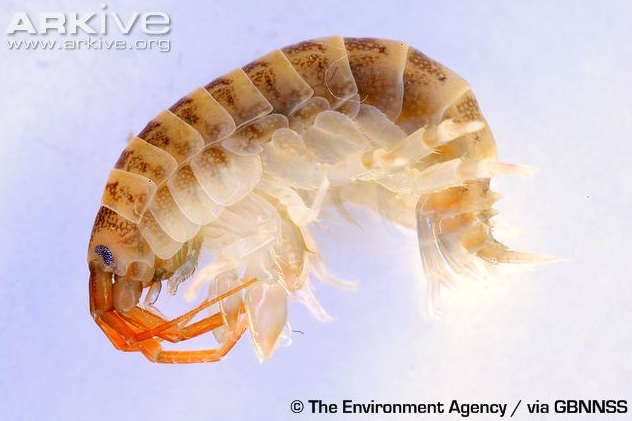
\includegraphics[width=8cm]{shrimpy2}}
\end{frame}

\begin{frame}{Killer Shrimp}
\centerline{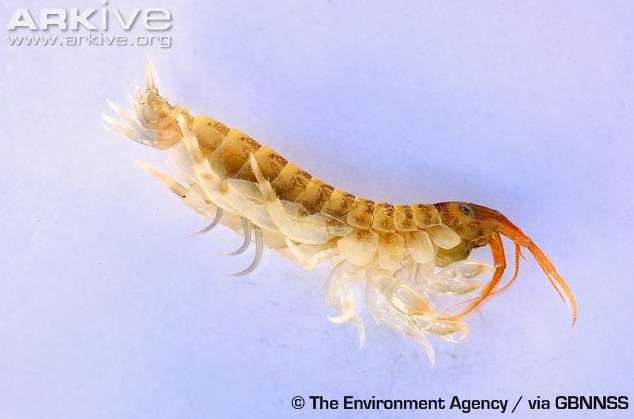
\includegraphics[width=8cm]{shrimpy3}}
\end{frame}

\begin{frame}
	\centerline{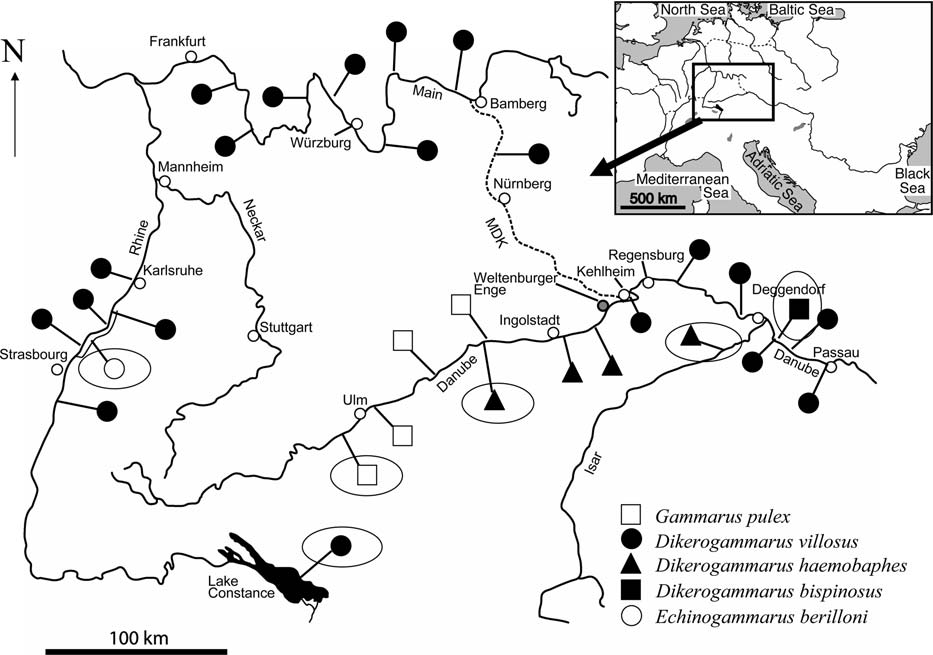
\includegraphics[width=10cm]{img/kinzlermap}}
	
	\center{(Kinzler, 2008)}
\end{frame}


\begin{frame}{Time Line}

  \vfill

  The time to prominence. 

  \vfill

  \begin{tabular}{l|l}
    Years      & Species \\ \hline
    $<$1976    & \textit{Gp} native\\
    1976-1994  & \textit{Dh} invades\\
    1992-1995  & \textit{Dv} invades, \textit{Dh} declines\\
    $>$1995    & All but \textit{Dv} coexist separate from \textit{Dv}
  \end{tabular}

  \vfill

\end{frame}

\begin{frame}
   \frametitle{Terminology}
	\begin{block}{Intraguild Predation}
		Mutual Predation\\
		Mutual Interference \\
	\end{block}
	\begin{block}{Intraspecific Predation}
		Cannibalism
	\end{block}
\end{frame}

\begin{frame}
   \frametitle{Kinzler, 2008 Study}
	\vfill
	
	Isolated pairs of specimens in a controlled environment
	\begin{itemize}
		\item One freshly moulted (prey) 
		\item One predator
		\item Total of 279 experiments
		\item Grouped by age, sex, and species
	\end{itemize}
	
\vfill
	Results\\
	\begin{itemize}
	\item Found \textit{Dv} to be clear strongest predator\\
\vspace{.5em}
	\item Found \textit{Dh} to have highest cannibalism rate
\end{itemize}

\vfill
\end{frame}

\begin{frame}
   \frametitle{Basic Goals}
\begin{center}
		{\Large{\textbf{Determine long term population trends!}}}\\


\vspace{2.5em}
		Does \textit{Dv} totally dominate in the end?\\
\vspace{.5em}
		Which species survive?\\
\vspace{.5em}

		Is there an equilibrium?

\end{center}

\end{frame}


%\begin{frame}
%  \frametitle{The Issues}
%
%  We gonna talk about the issues about talking about stuff.
%
%\end{frame}
%
%
%\begin{frame}
%  \frametitle{Random Stuff}
%
%  Random stuff is like totally out there.
%
%  \uncover<2->
%  {
%
%    It could just be totally surprising.
%
%  }
%
%  \uncover<3->
%  {
%
%    Unexpected even, you know what I mean?
%
%  }
%
%
%\end{frame}
%
%
%\subsection{Statistics}
%
%\begin{frame}{Statistics Do Not Lie}
%
%  You can totally trust the statistics.
%
%  \only<2>{
%
%    Well... usually
%    \begin{itemize}
%    \item We could make a type I error.
%    \item Or it could be a type II error.
%    \end{itemize}
%
%  }
%
%  \only<3-4>{
%
%    Then again maybe the hypothesis test does not even make sense.
%
%  }
%
%  \only<4->{
%
%    Then you are really hosed.
%
%  }
%
%\end{frame}




% %%%%%%%%%%%%%%%%%%%%%%%%%%%%%%%%%%%%%%%%%%%%%%%%%%%%%%%%%%%%
% %%%%% The specifics about modeling

\numberwithin{equation}{section}

\subsection{Nondimensionalization}
%\begin{frame}
  %\frametitle{Outline}
  %\tableofcontents[ currentsection ]
%\end{frame}

\begin{frame}
\frametitle{Nondimensionalization}

  The nondimensionalized system is:

	\begin{align*}
		\frac{dx}{dt} &= x^2 (1-x) - \alpha xy - \frac{\gamma_\circ x^2}{x+D}, \\
    \frac{dy}{dt} &= \rho y^2 (1-y) - \beta xy -\frac{\delta_\circ y^2}{y+R}
	\end{align*}
\end{frame}

\begin{frame}
  %\movie[height=6.33cm,width=8.55cm,loop,poster]{Milstein Process}{Milstein.mp4}
\end{frame}



\begin{frame}{Phase Plane}

  \vfill
	
  \begin{columns}
    \only<1> {
      \column{.65\textwidth}
      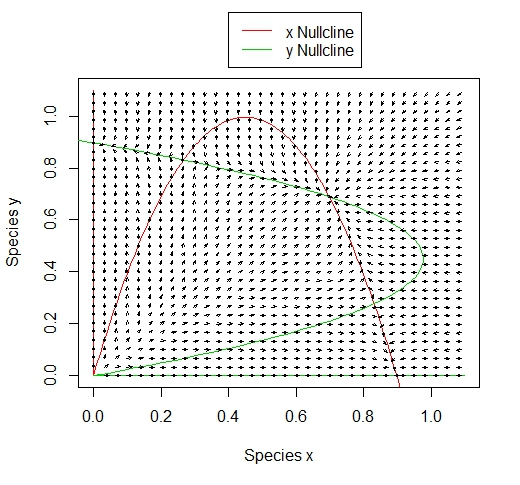
\includegraphics[height=7cm]{img/RplotMain}
      \column{.35\textwidth}
      $\alpha = .2, \beta = .2,
      \gamma = .8, \delta = .4, \rho = 1, R = 3$ and $D = 7$ 

      \begin{itemize}
      \item Six fixed points.
      \item Three are unstable.
      \end{itemize}
    }

    \only<2> {
      \column{.65\textwidth}
      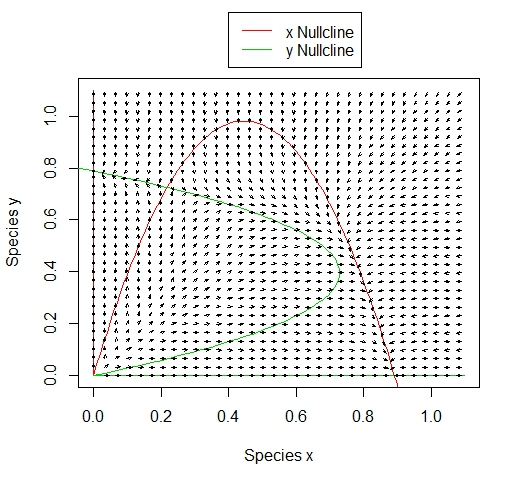
\includegraphics[height=7cm]{img/Rplot1} 
      \column{.35\textwidth}
      $\gamma = .85$ and $\delta = .8$ 
      \begin{itemize}
      \item Four fixed points.
      \item Two are unstable.
      \end{itemize}
    }

    \only<3> {
      \column{.65\textwidth}
      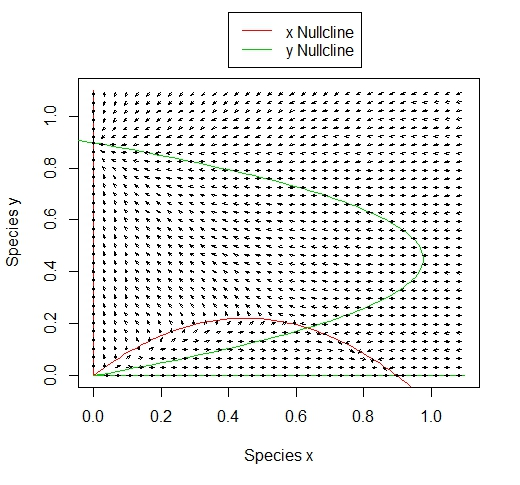
\includegraphics[height=7cm]{img/Rplot2} 
      \column{.35\textwidth}
      $\alpha = .9, \beta = .2, \gamma = .8$ and $\delta = .4$
      \begin{itemize}
      \item Four fixed points.
      \item Two are unstable.
      \end{itemize}
    }

    \only<4> {
      \column{.65\textwidth}
      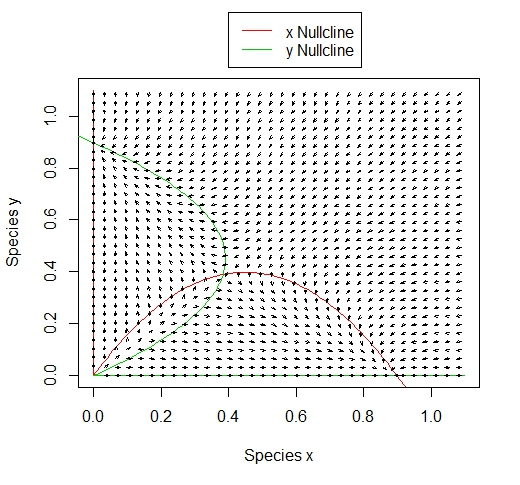
\includegraphics[height=7cm]{img/Rplot3} 
      \column{.35\textwidth}
      $\alpha = .5, \beta = .5, \gamma = .8$ and $\delta = .4$ 
      \begin{itemize}
      \item Four fixed points.
      \item Two are unstable.
      \end{itemize}
    }

    \only<5> {
      \column{.65\textwidth}
      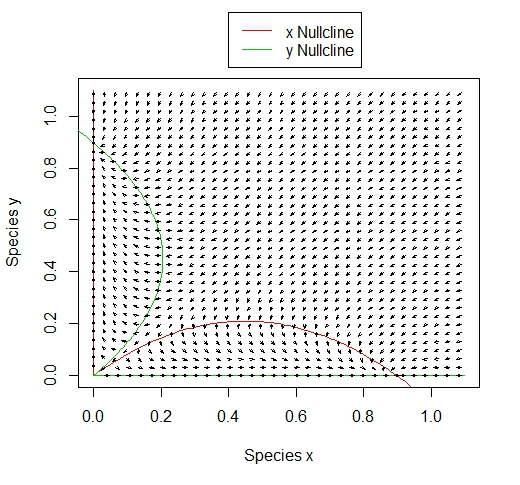
\includegraphics[height=7cm]{img/Rplot4} 
      \column{.35\textwidth}
      $\alpha = .95, \beta = .95, \gamma = .8$ and $\delta = .4$ 
      \begin{itemize}
      \item Three fixed points.
      \item One is unstable.
      \end{itemize}
    }

  \end{columns}
\end{frame}




\begin{frame}{Noise}

  Additive noise...
  \begin{align*}
    \frac{dx}{dt} &= x^2 (1-x) - \alpha xy - \frac{\gamma_\circ x^2}{x+D} + \upsilon \frac{dW}{dt}, \\
    \frac{dy}{dt} &= \rho y^2 (1-y) - \beta xy -\frac{\delta_\circ y^2}{y+R}+ \kappa \frac{dB}{dt}.
  \end{align*}

  Proportional noise...
  \begin{align*}
    \frac{dx}{dt} &= x^2 (1-x) - \alpha xy - \frac{\gamma_\circ x^2}{x+D} + \upsilon x \frac{dW}{dt}, \\
    \frac{dy}{dt} &= \rho y^2 (1-y) - \beta xy -\frac{\delta_\circ y^2}{y+R}+ \kappa y \frac{dB}{dt}.
  \end{align*}

\end{frame}


%
%
%\begin{frame}
%\frametitle{Heun's Method}
%\begin{itemize}
%\item Heun's method is a numerical procedure for approximating ordinary differential equations with a given initial value.
%\item First you calculate the intermediate value $\tilde{y}_{i+1}$ and then the final approximation $y_{i+1}$ at the next generation point.
%\end{itemize}
%
%\begin{align*}
%	\tilde{y}_{i+1} &= y_i + \Delta t \ f(t_i, y_i) \\
%	y_{i+1} &= y_i + \frac{\Delta t}{2} \left[f(y_i,t_i) + f(\tilde{y}_{i+1}, t_{i+1})\right]
%\end{align*}
%\end{frame}
%
%
%\begin{frame}
%   \frametitle{Heun's Method vs. Euler's Method - Simulation}
%For the DE $y'=r y$ on $[0,T]$,\\
%\vspace{1em}
%	%\hspace{1.5em} Heun's:$\hspace{1em} \tilde{y}_{i+1} = y_i + \Delta t \ f(t_i, y_i)$ \\
%		\hspace{1.5em} Heun's:$ \hspace{1em} y_{i+1} = y_i + \frac{\Delta t}{2} \left[f(y_i,t_i) + f(\tilde{y}_{i+1}, t_{i+1})\right]$ \vspace{1em} \\
%	\hspace{1.5em} Euler's:$\hspace{1em}\tilde{y}_{i+1} = y_i + \Delta t \ f(y_i, t_i)$ \\
%\begin{columns}[t]
%    \column{.5\textwidth} 
%    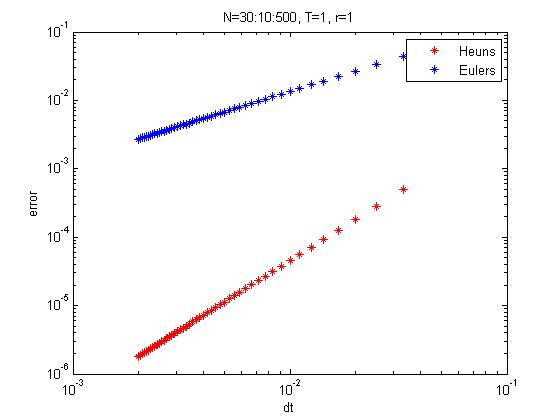
\includegraphics[width=6cm]{img/Heun500}
%    \column{.5\textwidth}
%    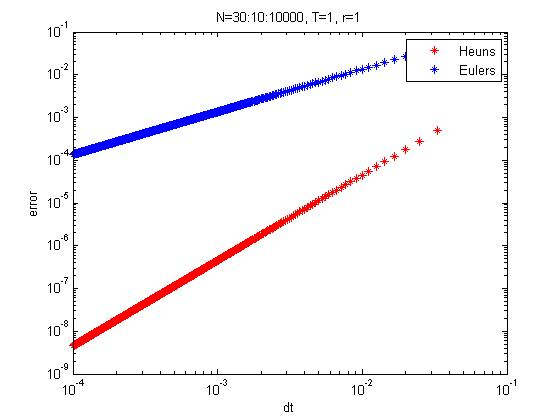
\includegraphics[width=6cm]{img/Heun10000}
%  \end{columns}
%
%\end{frame}



% %%%%%%%%%%%%%%%%%%%%%%%%%%%%%%%%%%%%%%%%%%%%%%%%%%%%%%%%%%%%
% %%%%% The specifics about SDEs



\numberwithin{equation}{section}

\section{Stochastic Calculus}
\begin{frame}
  \frametitle{Outline}
  \tableofcontents[ currentsection]
\end{frame}



\subsection{Stochastic Integration}

\begin{frame}
  \frametitle{Overview}

  The governing Equations:
  \begin{eqnarray*}
    \dot{a} & = & L_1a + N_1(a,g), \\
    \dot{g} & = & L_2g + N_2(a,g).
  \end{eqnarray*}


\end{frame}

\begin{frame}
	\frametitle{Calculating Stochastic Integrals}
		As an example consider the integral 
			$$Z_t=\int_0^t B(s) dB(s)$$
			
		This integral can be calculated as
			$$\displaystyle \int_0^t B(s)dB(s)=\frac{1}{2}(B^2(t)-B^2(0))-\frac{1}{2}$$
			
			% % can go over this calculation during presentation using Taylor Expansion
			
\end{frame}





\begin{frame}
  \frametitle{The ``Usual Scaling''}
  \begin{eqnarray*}
    x & \rightarrow & \bar{X} \xi, \\
    t & \rightarrow & \bar{T} s.
  \end{eqnarray*}

\end{frame}

%\begin{frame}
  %\frametitle{The Finite Difference Approximation}

  %\begin{itemize}
  %\item<4-> Usual stability issues.
  %\item<3-> Usual ease of use.
  %\item<2-> Usual wave speed problem.
  %\item<1-2> Usual centered difference scheme.
  %\end{itemize}
  %\uncover<3->{Don't that beat all?}

%\end{frame}


\subsection{Stochastic Differential Equations}

%\begin{frame}
 % \frametitle{Comparison}

  %\begin{columns}[t]
   % \column{.5\textwidth}
    %\centerline{\includegraphics[height=5.0cm]{gainComp-001}}
    %This is what the left looks like

    %\column{.5\textwidth}
    %\centerline{\includegraphics[height=5.0cm]{energyComp-001}}
    %This is what the right looks like

  %\end{columns}

%\end{frame}


%\subsection{Random Thoughts}
%\begin{frame}
 % \frametitle{Random Thoughts}
  %But what about Barney and PBS?

  %\begin{columns}[t]
    
   % \column{.5\textwidth}
    %\begin{block}{Barney?}
     % Is it okay to trust your kids with Barney?
    %\end{block}
    %\pause
  
    %\column{.5\textwidth}
    %\begin{block}{No, not Barney!}
     % Probably not.
    %\end{block}

  %\end{columns}


%\end{frame}





\end{document}

